\documentclass[10pt,twoside]{scrreprt}

\renewcommand{\textfraction}{0.001}
\renewcommand{\topfraction}{0.999}   
\renewcommand{\bottomfraction}{0.999}

\usepackage{graphicx}
\usepackage{amsmath}
\usepackage{amssymb}
\usepackage[bibencoding=utf8, backend=biber, style=numeric, minbibnames=1, maxnames=5]{biblatex}
\addbibresource{bibliography.bib}
\usepackage{a4,color}
\usepackage{tikz}

\usepackage{booktabs}
\usepackage{caption}
\usepackage{float}
\usepackage{url}

\usepackage[T1]{fontenc}
\usepackage[utf8]{inputenc}

\usepackage{mathpazo}

\definecolor{red}{rgb}{1,0,0}
\definecolor{green}{rgb}{0,1,0}
\definecolor{blue}{rgb}{0,0,1}
\definecolor{darkblue}{rgb}{0,0,0.8}

\definecolor{yellow}{rgb}{1,1,0}
\definecolor{lightblue}{rgb}{0,1,1}
\definecolor{magenta}{rgb}{1,0,1}
\definecolor{lightgrey}{rgb}{0.5,0.5,0.5}
\definecolor{grey}{rgb}{0.35,0.35,0.35}
\definecolor{darkgrey}{rgb}{0.2,0.2,0.2}
\definecolor{ockerrot}{rgb}{0.859,0.375,0.152}


\captionsetup{margin=0pt,font=small,labelfont=sc,labelformat=simple,format=plain,indention=3mm,
 labelsep=endash,textfont=sf,font=sf,singlelinecheck=on,figurename=Fig.,tablename=Tab.}


\fontfamily{ppl}\selectfont


\begin{document}

\chapter*{Abstract}
\addcontentsline{toc}{chapter}{Abstract}
Abstract stuff
	

\chapter{Introduction}
\section{LHC - Large Hadron Collider} % (fold)
\label{sec:lhc_large_hadron_collider}

The Large Hadron Collider (LHC) is the world's largest particle collider ever built. 

% section lhc_large_hadron_collider (end)

\chapter{Theory}

\section{RICH Detector} % (fold)
\label{sec:rich_detector}

Particle identification is a fundamental requirement at the LHCb experiment. Meaningful CP-violation measurements are only possible if hadron identification is available hence the ability to distinguish between kaons and pions is  essential.
% section rich_detector (end)

\section{Cherenkov-Radiation} % (fold)
\label{sec:cherenkov_radiation}

The speed of light in vacuum, \( \mathbf{c} \), is a universal physical constant. According to Einstein's special theory of relativity, \( c \) is the maximum speed at which all matter (or information) in the universe can travel. The speed at which light propagates in a medium, however, can be significantly less can \( c \).

Cherenkov radiation results when a charged particle travels through a dielectric medium with a speed greather than the speed of light through said medium. Moreover, the velocity that must be exceeded is the phase velocity (\( v_{\text{Phase}} \text{ or short } v_{\text{P}} \)) and not the group velocity \( v_{\text{Group}} = \frac{\partial \omega}{\partial k} \).

\[ v_{\text{Phase}} = \frac{\lambda}{T} \quad \text{or} \quad \frac{\omega}{k}\]

As a charged particle travels through the medium, it disrupts the local electromagnetic field. If the particle travels slowly then the disturbance elastically relaxes to the mechinal equilibrium as the particle passes. However, if the particle travels fast enough, the limited response speed of the medium means that a disturbance is left in the wake of the particle, and the energy in this disturbance radiates as coherent shockwave.

\begin{figure}[htbp]
	\centering
		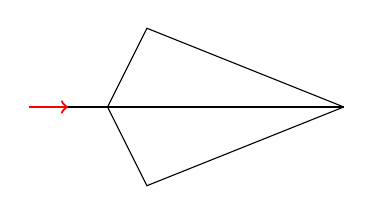
\begin{tikzpicture}
			\draw (-1,0) -- (3,0);
			\draw (0,0) -- (0.5,1) -- (3,0);
			\draw (0,0) -- (0.5,-1) -- (3,0);
			\draw[->, red, thick] (-1,0) -- (-0.5,0);
		\end{tikzpicture}
	\caption{Cherenkov radiation}
	\label{fig:label}
\end{figure}

\begin{align}
    x_p &= v_{p}\cdot t = \beta c t \nonumber \\
    x_{\text{em}} &= v_{\text{em}}\cdot t=\frac{c}{n}t \nonumber \\
    \cos\theta &= \frac{x_{\text{p}}}{x_{\text{em}}} = \frac{\frac{c}{n}t}{\beta c t} = \frac{1}{n\beta} \nonumber
\end{align}

which is independent from the angle \( \theta \).
% section cherenkov_radiation (end)

\section{Hough Transform} % (fold)
\label{sec:hough_transform}

The Hough-Transform is a feature extraction technique used in image analysis, computer vision and digital image processing.

the purpose is to find imperfect instances of objects within a certain cass of shapes by a voting procedure. This voting procedure is carried out in a parameter space from which object candidates are obtained as local maxima in a so called accumlator space that is explicitly constructed by the algorithm for computing the Hough-Transform.

Initially the Hough-Transform was concerned with finding straight lines but has been extended to identifying positions of arbitrary shapes, such as circles and ellipses.

\subsection{Linear Hough Transform} % (fold)
\label{sub:linear_hough_transform}

A linear function is normally defined as the following:

\[
  f(x) = m\cdot x + b
\]
where $m$ is the slope of the line and $b$ the intercept. For the Hough-Transform however, this representation is not ideal. For a vertical line $m$ would go to infinity which gives us an unbound transform space for $m$. For this reason Duda and Hart suggested the $\rho\text{-}\theta$ parametrization \parencite{Duda:1972}.

\[
  r = x\cos\theta + y\sin\theta
\]
where $r$ is the distance from the origin to the closest point in the line and $\theta$ is the angle between the $x$-axis and the line connecting the origin with that closest point.

\begin{figure}[h]
  \centering
  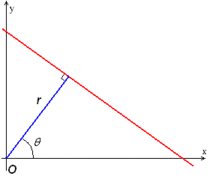
\includegraphics[width=0.3\textwidth]{pics/R_theta_line.png}
  \caption{$\rho\text{-}\theta$ parametrisation}
  \label{fig:rhotheta}
\end{figure}
% subsection linear_hough_transform (end)

This means given a single point in the plane, the set of all lines going through this point form a sinusoidal curve in $\rho\text{-}\theta$ space. Another point 
that lies on the same straight line in the plane will produce a sinusoidal curve that intersects with the other at ($\rho\text{-}\theta$).

\subsubsection{Example of a Linear HT} % (fold)
\label{ssub:example_of_a_linear_ht}

\begin{tikzpicture}
  \draw[<->] (3,0) -- (0,0) -- (0,3);

  \foreach \x in {0,0.5,1} {
    \draw[fill] (2-\x, 2-\x) circle (1pt);
  }
\end{tikzpicture}
\begin{table}
\centering
\caption{Angle vs Distance}
\begin{tabular}{rr}
\toprule
 Angle & Distance \\
\midrule
0 & 2.334 \\
\bottomrule
\end{tabular}
\end{table}

% subsubsection example_of_a_linear_ht (end)


\subsection{Circle Hough Transform} % (fold)
\label{sub:circle_hough_transform}

For this thesis we are interested in circle detection so we need to adapt our linear Hough Transform in order to find circles. In a two dimensional space, a circle can be described by:

\begin{equation}
		(x-c_x)^2 + (y-c_y)^2 = r^2
\end{equation}

Where $(c_x,c_y)$ is the center of the circle and $r$ the radius. The possible parameters for the parameters space are now $c_x, c_y$ and $r$. This means if we know the center of the circle the parameter space is one-dimensional and if we know the radius of the circle our parameter space is two-dimensional and of course if we know nothing the parameter space is three-dimensional.

% subsection circle_hough_transform (end)

\subsection{Combinatorial Approach} % (fold)
\label{sub:combinatorial_approach}

This approach is slightly different from the usual Hough Transforms. In this approach we use the fact that a circle is uniquely defined by 3 points.

% subsection combinatorial_approach (end)
% section hough_transform (end)


\chapter{Methods}

\section{Conventional Hough-Transforms} % (fold)
\label{sec:conventional_hough_transforms}

% section conventional_hough_transforms (end)

\subsection{1D: Known Center - Find Radius} % (fold)
\label{sub:1d_known_center_find_radius}



% subsection 1d_known_center_find_radius (end)
\subsection{2D: Known Radius - Find Center} % (fold)
\label{sub:2d_known_radius_find_center}

% section 2d_known_radius_find_center (end)

\subsection{3D: Nothing is Known - Find Everything} % (fold)
\label{sub:3d_nothing_is_known_find_everything}

% subsection 3d_nothing_is_known_find_everything (end)

\section{Combinatorial approach}

The combinatorial approach relies on the fact that a circle is uniquely defined by 3 points. With 2 arbotrary points we couldn't tell which side the circle is
going to go. A third point gives us all the information we need. The general idea then is the following:

\begin{enumerate}
\item Build all possible triples of points given the data points
\item For all the point triples calculate the center and the radius of the potential circle
\item Due to constraints in the radius we can drop many of the circles with a radius bigger than a certain threshold
\item Create a histogram with the radius distribution. Peaks in the radius distribution hint to a circle.
\item We scan the radius histogram for peaks and look at the center point histogram for the given radius of a peak. If we have also a peak in the center point histogram
      the set of the points of the triples lie on a circle with a radius and center given by the histogram peaks.
\end{enumerate}

\subsection{Drawback}
	

There is also a drawback with this method:

\begin{itemize}
\item The combinatorics blow up with a high number of data points \( \binom{N}{3} \)
\end{itemize}

So for example with 200 data points (circle data and background) the number of triplets is

\[ \binom{200}{3} = 1313400 \]

and for 300:

\[ \binom{300}{3} = 4455100 \]


\begin{figure}[tb]
  \centering
  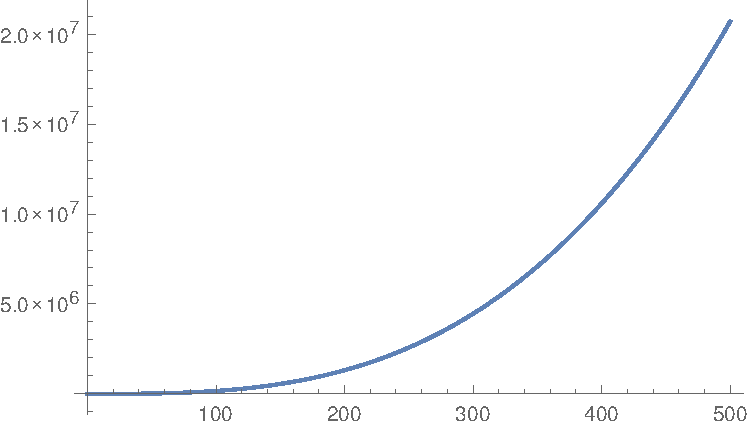
\includegraphics[width=0.5\textwidth]{pics/binomial_growth}
  \caption{Binomial Growth with $\binom{N}{3}$}
  \label{fig:figure1}
\end{figure}

\chapter{Results}


\chapter{Conclusions} % (fold)
\label{cha:conclusions}

% chapter conclusions (end)

\printbibliography
\end{document}